\documentclass[11pt]{article}

\usepackage[letterpaper,margin=0.82in]{geometry}
\usepackage[T1]{fontenc}
\usepackage{lmodern}
\usepackage{microtype}
\usepackage{amsmath,amssymb,bm}
\usepackage{graphicx}
\usepackage{booktabs}
\usepackage{array}
\usepackage{siunitx}
\usepackage{caption}
\usepackage{subcaption}
\usepackage{enumitem}
\usepackage{float}
\usepackage{xcolor}
\usepackage{fancyhdr}
\usepackage{hyperref}
\usepackage{listings}
\usepackage{setspace}

\definecolor{navy}{RGB}{24,52,93}
\definecolor{graytext}{RGB}{90,90,90}
\definecolor{codebg}{RGB}{247,248,250}

\hypersetup{
    colorlinks=true,
    linkcolor=navy,
    citecolor=navy,
    urlcolor=navy,
    pdftitle={Gyroscope Dynamics Simulation and Experimental Validation},
    pdfauthor={Jeonghyun Park, Sam Seaberry, Katherine Tao}
}

\pagestyle{fancy}
\setlength{\headheight}{14pt}
\fancyhf{}
\lhead{Gyroscope Dynamics Simulation}
\rhead{Experimental Validation}
\cfoot{\thepage}
\renewcommand{\headrulewidth}{0.4pt}

\captionsetup{font=small,labelfont=bf}
\setlist[itemize]{leftmargin=1.35em,itemsep=0.25em,topsep=0.4em}
\setstretch{1.05}
\sisetup{per-mode=symbol}

\lstset{
    basicstyle=\ttfamily\small,
    backgroundcolor=\color{codebg},
    frame=single,
    rulecolor=\color{black!15},
    breaklines=true,
    columns=fullflexible,
    showstringspaces=false
}

\newcommand{\vect}[1]{\bm{#1}}
\newcommand{\mat}[1]{\bm{#1}}
\newcommand{\R}{\mat{R}}

\begin{document}
\hypersetup{pageanchor=false}

\begin{titlepage}
    \centering
    \vspace*{1.0in}
    {\Large\color{navy}\textbf{GYROSCOPE DYNAMICS SIMULATION AND EXPERIMENTAL VALIDATION}\par}
    \vspace{0.25in}
    {\large A Newton--Euler rigid-body model implemented in MATLAB\par}
    \vspace{0.7in}
    \rule{0.82\textwidth}{0.8pt}\par
    \vspace{0.45in}
    {\large Jeonghyun Park \quad Sam Seaberry \quad Katherine Tao\par}
    \vspace{0.15in}
    {\normalsize MCEN90038 Dynamics, University of Melbourne\par}
    {\normalsize May 2026\par}
    \vfill
    \begin{minipage}{0.82\textwidth}
    \vspace{0.5in}
\end{titlepage}
\clearpage
\pagenumbering{roman}
\hypersetup{pageanchor=true}
\begin{abstract}
This project develops a three-degree-of-freedom rigid-body model of a laboratory gyroscope and compares its predicted motion with measurements from a sensor mounted on the gyroscope bar. The model represents base precession, bar tilt, and rotor spin through a sequence of rotation matrices, constructs body inertia tensors with cylindrical cutouts, transfers those inertias to the pivot by the parallel-axis theorem, and applies Newton--Euler angular-momentum balance to obtain nonlinear equations of motion. The resulting symbolic equations are converted to numerical functions and integrated in MATLAB using \texttt{ode45}. Simulated angular velocity and sensor acceleration are transformed into the sensor frame and compared against measured signals over short and long time windows. The model reproduces the principal direction and oscillatory structure of gyroscopic precession and nutation, while systematic discrepancies remain because the model neglects friction and drag, approximates some geometry, and uses an estimated initial rotor speed. These differences provide a clear boundary between ideal rigid-body dynamics and the measured behavior of the physical apparatus.
\end{abstract}

\setcounter{tocdepth}{1}
\tableofcontents
\clearpage
\pagenumbering{arabic}

\section{Introduction}
A spinning rigid body tends to preserve the direction of its angular momentum in the absence of external torque. When a torque acts transverse to the existing angular momentum, the rotational axis changes direction rather than simply rotating about the applied-torque axis. This behavior is the basis of gyroscopic precession and appears in inertial-navigation systems, vehicle dynamics, spacecraft attitude systems, and classical dynamics demonstrations \cite{openstax_precession,kostov2011}.

The apparatus studied here consists of an unbalanced horizontal bar that can tilt and precess about a support, with counterweights on one side and a rapidly spinning rotor on the other. Gravity therefore applies a persistent external moment about the pivot. The engineering objective is not merely to reproduce the familiar qualitative gyroscope motion, but to construct a model that predicts measurable angular velocities and accelerations at the location of an onboard sensor.

The work is organized around four tasks:
\begin{itemize}
    \item define a consistent sequence of inertial and body-fixed reference frames;
    \item construct the mass and inertia properties of the rotor and counterweights;
    \item derive and numerically integrate the nonlinear equations of motion; and
    \item transform the simulated states into the sensor frame for comparison with experiment.
\end{itemize}

\section{Physical System and Modeling Assumptions}
\subsection{Coordinate description}
The kinematic model uses three generalized coordinates:
\begin{align}
    \beta(t) &:\quad \text{precession about the inertial vertical axis},\\
    \theta(t) &:\quad \text{tilt of the main bar},\\
    \alpha(t) &:\quad \text{spin of the rotor about its own axis}.
\end{align}
The original project diagram is reproduced in Figure~\ref{fig:kinematic}. Point $B$ is the principal pivot and serves as the reference point for the rigid-body angular-momentum balance. Point $A$ lies near the rotor-side joint, and the sensor is rigidly attached to the main bar.

\begin{figure}[H]
    \centering
    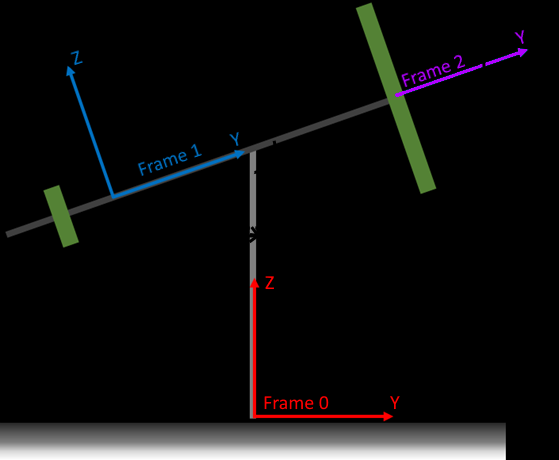
\includegraphics[width=0.66\textwidth]{figures/system_kinematic_model.png}
    \caption{Kinematic model and reference-frame layout used in the original project. Frame 0 is inertial; the successive body frames represent base precession, bar tilt, and rotor spin.}
    \label{fig:kinematic}
\end{figure}

\subsection{Assumptions}
The model intentionally idealizes the apparatus so that the dominant gyroscopic dynamics can be isolated. The principal assumptions are:
\begin{itemize}
    \item the connecting rod is massless;
    \item the rotor, pulley, and counterweights are represented as cylinders with central rod cutouts;
    \item gravitational acceleration is constant at $g=\SI{9.80665}{m/s^2}$;
    \item bearing friction and aerodynamic drag are neglected;
    \item bodies are rigid and connections do not deform;
    \item the sensor is represented by a fixed position vector on the main bar; and
    \item the combined rotor-pulley center location is approximated from the measured component offsets.
\end{itemize}
The frictionless assumption is especially important when interpreting the long-duration comparison because the real rotor loses energy while the simulation does not.

\section{Kinematics}
\subsection{Rotation matrices}
The MATLAB implementation applies successive rotations about the inertial $z$ axis, the intermediate $x$ axis, and the rotor $y$ axis. With $c_q=\cos q$ and $s_q=\sin q$,
\begin{align}
\R_{10}(\beta) &=
\begin{bmatrix}
 c_\beta & -s_\beta & 0\\
 s_\beta &  c_\beta & 0\\
 0 & 0 & 1
\end{bmatrix},\\[4pt]
\R_{21}(\theta) &=
\begin{bmatrix}
1 & 0 & 0\\
0 & c_\theta & -s_\theta\\
0 & s_\theta & c_\theta
\end{bmatrix},\\[4pt]
\R_{32}(\alpha) &=
\begin{bmatrix}
 c_\alpha & 0 & s_\alpha\\
 0 & 1 & 0\\
 -s_\alpha & 0 & c_\alpha
\end{bmatrix}.
\end{align}
The full orientations relative to the inertial frame are
\begin{equation}
    \R_{20}=\R_{10}\R_{21}, \qquad
    \R_{30}=\R_{10}\R_{21}\R_{32}.
\end{equation}
This formulation keeps the coordinate transforms explicit and allows position, inertia, angular momentum, and sensor measurements to be expressed consistently.

\subsection{Angular velocity}
The angular velocity of frame 2, expressed in frame 2, follows directly from the precession and tilt rates:
\begin{equation}
\vect{\omega}_{2}^{(2)}=
\begin{bmatrix}
\dot{\theta}\\
\dot{\beta}\sin\theta\\
\dot{\beta}\cos\theta
\end{bmatrix}.
\label{eq:omega2}
\end{equation}
The rotor frame additionally includes the spin rate $\dot{\alpha}$:
\begin{equation}
    \vect{\omega}_{3}^{(3)}
    = \R_{32}^{T}\vect{\omega}_{2}^{(2)}
    + \begin{bmatrix}0 & \dot{\alpha} & 0\end{bmatrix}^{T}.
\end{equation}
Equation~\eqref{eq:omega2} later provides the simulated angular velocity that is compared directly with the sensor output.

\section{Mass Properties and Rigid-Body Dynamics}
\subsection{Cylinder inertia with central cutout}
Each major component is approximated as a cylinder whose symmetry axis is aligned with the local $y$ direction. The inertia tensor at the cylinder center of mass is
\begin{equation}
\mat{I}_{\mathrm{cyl}}=
\begin{bmatrix}
\frac{1}{4}mR^2+\frac{1}{12}mL^2 & 0 & 0\\
0 & \frac{1}{2}mR^2 & 0\\
0 & 0 & \frac{1}{4}mR^2+\frac{1}{12}mL^2
\end{bmatrix}.
\end{equation}
Because the mounting rod passes through each component, the inertia of the cylindrical hole is subtracted. The hole mass is obtained from the parent-body density,
\begin{equation}
    \rho=\frac{m}{\pi R^2L}, \qquad
    m_{\mathrm{hole}}=\rho\,\pi r_{\mathrm{hole}}^2L.
\end{equation}

\subsection{Transfer to the pivot}
For a body whose center is offset from point $B$ by vector $\vect{r}$, the parallel-axis theorem gives
\begin{equation}
    \mat{I}_{B}=\mat{I}_{C}+m\left[(\vect{r}^{T}\vect{r})\mat{1}-\vect{r}\vect{r}^{T}\right].
\end{equation}
The same operation is applied to the solid body and its cylindrical cutout; the net inertia is obtained by subtraction. This produces pivot-referenced inertia tensors for the two counterweights and the rotor-pulley assembly.

\subsection{Angular-momentum balance}
For each rigid body,
\begin{equation}
    \vect{H}_{B}=\mat{I}_{B}\vect{\omega}.
\end{equation}
Because the vector is represented in a rotating body frame, its inertial derivative uses the transport theorem,
\begin{equation}
    \left(\frac{d\vect{H}}{dt}\right)_{0}
    =\left(\frac{d\vect{H}}{dt}\right)_{\mathrm{body}}
    +\vect{\omega}\times\vect{H}.
\label{eq:transport}
\end{equation}
Gravitational moments and the moment transmitted from the rotor side are combined with Equation~\eqref{eq:transport} to form the nonlinear equations of motion. In symbolic form, the implementation is rearranged as
\begin{equation}
    \mat{A}(\vect{q})\,\ddot{\vect{q}}
    = \vect{b}(\vect{q},\dot{\vect{q}}),
    \qquad
    \vect{q}=\begin{bmatrix}\beta&\theta&\alpha\end{bmatrix}^{T}.
\label{eq:mass_matrix}
\end{equation}
Rather than printing the very large closed-form expressions, the MATLAB workflow extracts the mass matrix and forcing vector symbolically and converts the solved accelerations into numerical functions.

\section{Numerical Implementation}
The simulation pipeline is summarized below:
\begin{enumerate}[leftmargin=1.55em,itemsep=0.35em]
    \item declare symbolic generalized coordinates and rotation matrices;
    \item define measured geometry and component mass properties;
    \item construct pivot-referenced inertia tensors;
    \item form angular momentum and its rotating-frame derivative;
    \item assemble the equations of motion and solve symbolically for $\ddot{\beta}$, $\ddot{\theta}$, and $\ddot{\alpha}$;
    \item convert those expressions to numerical MATLAB functions;
    \item integrate the six-state first-order system with \texttt{ode45}; and
    \item reconstruct sensor-frame angular velocity and acceleration for validation.
\end{enumerate}

The state vector is
\begin{equation}
    \vect{x}=\begin{bmatrix}
    \beta & \theta & \alpha & \dot{\beta} & \dot{\theta} & \dot{\alpha}
    \end{bmatrix}^{T},
\end{equation}
with time derivative
\begin{equation}
    \dot{\vect{x}}=\begin{bmatrix}
    \dot{\beta} & \dot{\theta} & \dot{\alpha} &
    \ddot{\beta} & \ddot{\theta} & \ddot{\alpha}
    \end{bmatrix}^{T}.
\end{equation}
The model is integrated for \SI{90}{s} with relative and absolute tolerances of $10^{-7}$.

\subsection{Model parameters}
Table~\ref{tab:params} collects the primary numerical values used in the supplied MATLAB source.

\begin{table}[H]
\centering
\caption{Principal model parameters from the MATLAB implementation.}
\label{tab:params}
\begin{tabular}{>{\raggedright\arraybackslash}p{0.43\textwidth} S[table-format=1.5] l}
\toprule
\textbf{Quantity} & {\textbf{Value}} & \textbf{Unit} \\
\midrule
Large counterweight mass & 0.900 & kg \\
Small counterweight mass & 0.030 & kg \\
Rotor + pulley mass & 1.470 & kg \\
Large counterweight radius & 0.035 & m \\
Small counterweight radius & 0.022 & m \\
Rotor radius & 0.127 & m \\
Pulley radius & 0.0291 & m \\
Counterweight hole radius & 0.0128 & m \\
Rotor hole radius & 0.0093 & m \\
Large counterweight offset from pivot & -0.310 & m \\
Small counterweight offset from pivot & -0.282 & m \\
Approx. rotor-pulley center offset & 0.150775 & m \\
\bottomrule
\end{tabular}
\end{table}

\section{Experimental Validation}
\subsection{Initial conditions}
The initial rotor speed was estimated from tachometer measurements at approximately \SI{500}{rpm}, corresponding to
\begin{equation}
    \dot{\alpha}_0 = 500\frac{2\pi}{60}
    \approx \SI{52.36}{rad/s}.
\end{equation}
The bar tilt was initialized at $\theta_0=15^{\circ}$ under the model's coordinate convention. Other generalized coordinates and angular rates were initialized at zero.

\subsection{Sensor-frame acceleration}
The experimental sensor is rigidly mounted to the main bar. For a sensor at position $\vect{r}_{B/S}$ relative to pivot $B$, rigid-body acceleration is reconstructed from
\begin{equation}
    \vect{a}_{S}
    = \vect{\alpha}_2\times\vect{r}_{B/S}
    + \vect{\omega}_2\times\left(\vect{\omega}_2\times\vect{r}_{B/S}\right)
    - \R_{20}^{T}\vect{g}.
\label{eq:sensoracc}
\end{equation}
The first term is tangential acceleration, the second is centripetal acceleration, and the final term expresses gravitational acceleration in the sensor/body frame. The supplied implementation uses
\begin{equation}
    \vect{r}_{B/S}=\begin{bmatrix}0&-0.15&0.05\end{bmatrix}^{T}\;\mathrm{m}.
\end{equation}

\subsection{Reproducibility note}
The revised report was prepared from the original PDF and MATLAB source provided for this portfolio update. The experimental CSV itself was not included among those files. Consequently, the figures below preserve the original model-versus-measurement plots, but new quantitative error metrics such as RMSE, phase lag, or confidence intervals are not invented here. Those metrics should be recomputed once the raw sensor export is added to the repository.

\section{Results}
\subsection{Angular velocity}
Figures~\ref{fig:wx}--\ref{fig:wz} compare measured and modeled angular-velocity components. The short-time plots make phase and amplitude correspondence visible; the \SI{90}{s} plots show the accumulated period mismatch and the absence of dissipative decay in the ideal model.

\begin{figure}[H]
\centering
\begin{subfigure}[t]{0.49\textwidth}
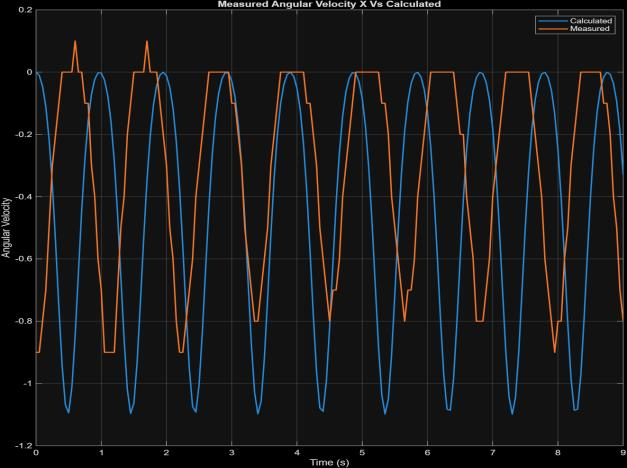
\includegraphics[width=\textwidth]{figures/angular_velocity_x_9s.png}
\caption{First \SI{9}{s}.}
\end{subfigure}\hfill
\begin{subfigure}[t]{0.49\textwidth}
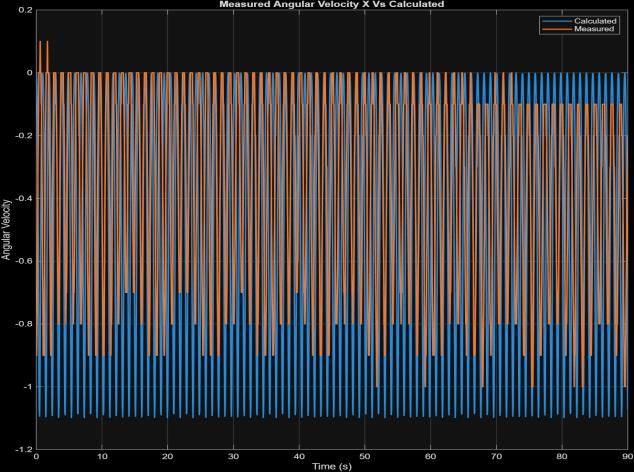
\includegraphics[width=\textwidth]{figures/angular_velocity_x_90s.png}
\caption{Full \SI{90}{s}.}
\end{subfigure}
\caption{Measured and calculated angular velocity, sensor $x$ channel.}
\label{fig:wx}
\end{figure}

\begin{figure}[H]
\centering
\begin{subfigure}[t]{0.49\textwidth}
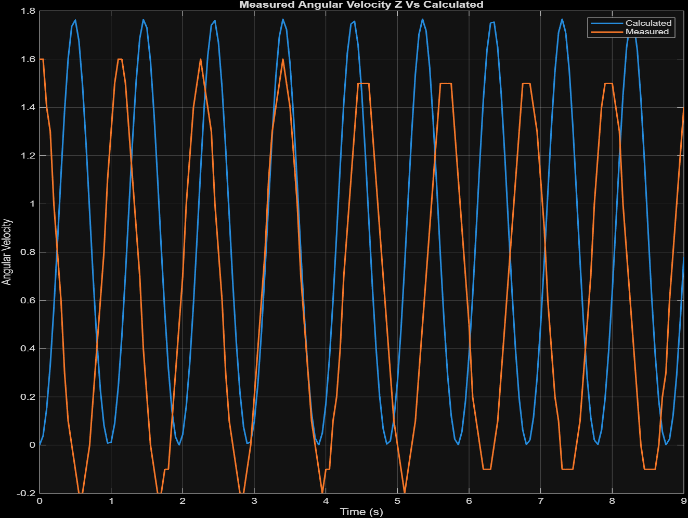
\includegraphics[width=\textwidth]{figures/angular_velocity_y_9s.png}
\caption{First \SI{9}{s}.}
\end{subfigure}\hfill
\begin{subfigure}[t]{0.49\textwidth}
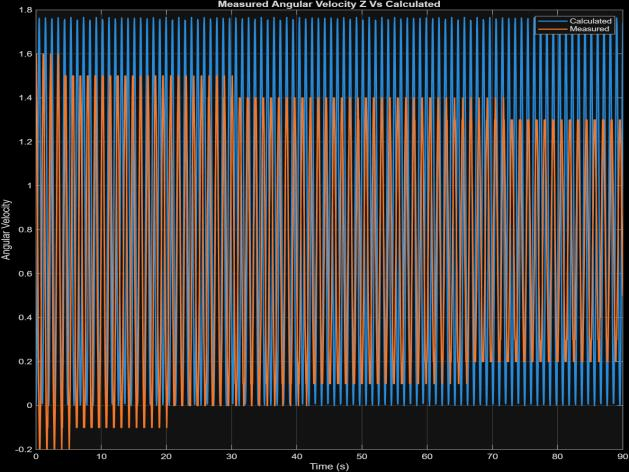
\includegraphics[width=\textwidth]{figures/angular_velocity_y_90s.png}
\caption{Full \SI{90}{s}.}
\end{subfigure}
\caption{Measured and calculated angular velocity, sensor $y$ channel.}
\label{fig:wy}
\end{figure}

\begin{figure}[H]
\centering
\begin{subfigure}[t]{0.49\textwidth}
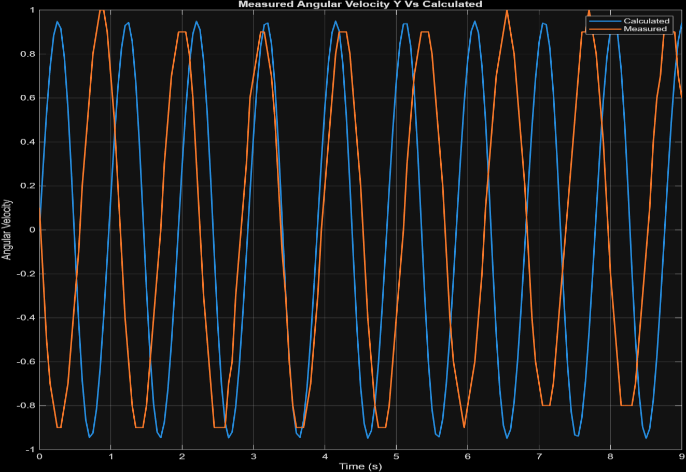
\includegraphics[width=\textwidth]{figures/angular_velocity_z_9s.png}
\caption{First \SI{9}{s}.}
\end{subfigure}\hfill
\begin{subfigure}[t]{0.49\textwidth}
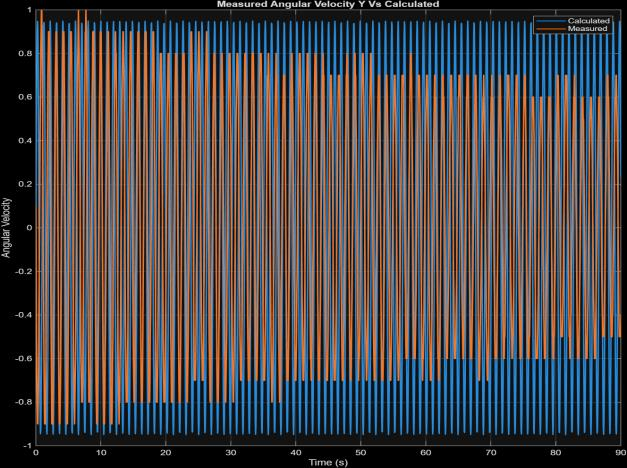
\includegraphics[width=\textwidth]{figures/angular_velocity_z_90s.png}
\caption{Full \SI{90}{s}.}
\end{subfigure}
\caption{Measured and calculated angular velocity, sensor $z$ channel.}
\label{fig:wz}
\end{figure}

\subsection{Linear acceleration}
The acceleration comparisons are shown in Figures~\ref{fig:ax}--\ref{fig:az}. The short-window curves preserve the primary periodic structure predicted by rigid-body kinematics. Over longer durations, the experimental signals display additional drift, decay, and low-frequency structure that the idealized model does not reproduce.

\begin{figure}[H]
\centering
\begin{subfigure}[t]{0.49\textwidth}
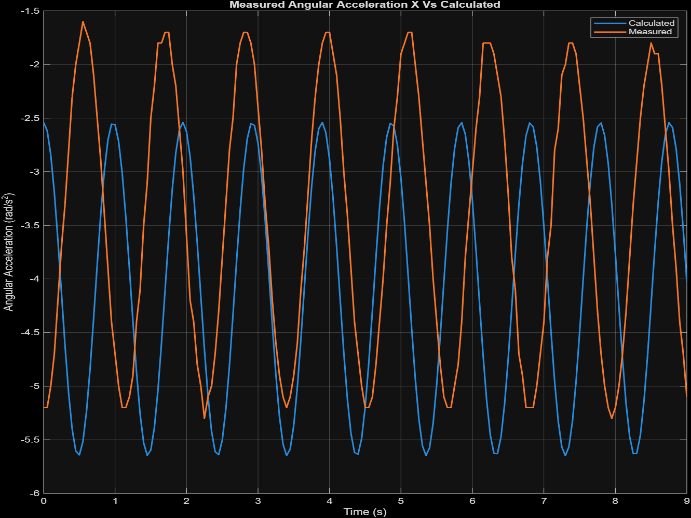
\includegraphics[width=\textwidth]{figures/acceleration_x_9s.png}
\caption{First \SI{9}{s}.}
\end{subfigure}\hfill
\begin{subfigure}[t]{0.49\textwidth}
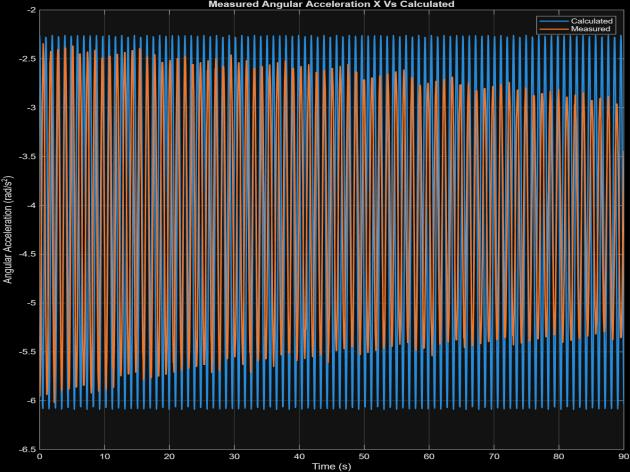
\includegraphics[width=\textwidth]{figures/acceleration_x_90s.png}
\caption{Full \SI{90}{s}.}
\end{subfigure}
\caption{Measured and calculated linear acceleration, sensor $x$ channel.}
\label{fig:ax}
\end{figure}

\begin{figure}[H]
\centering
\begin{subfigure}[t]{0.49\textwidth}
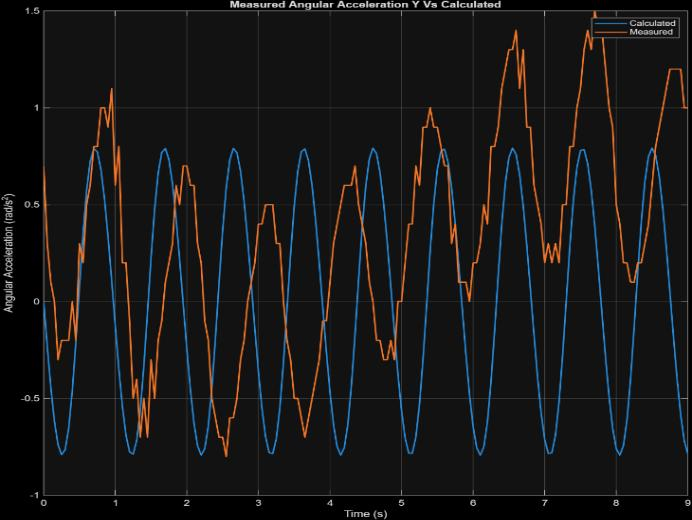
\includegraphics[width=\textwidth]{figures/acceleration_y_9s.png}
\caption{First \SI{9}{s}.}
\end{subfigure}\hfill
\begin{subfigure}[t]{0.49\textwidth}
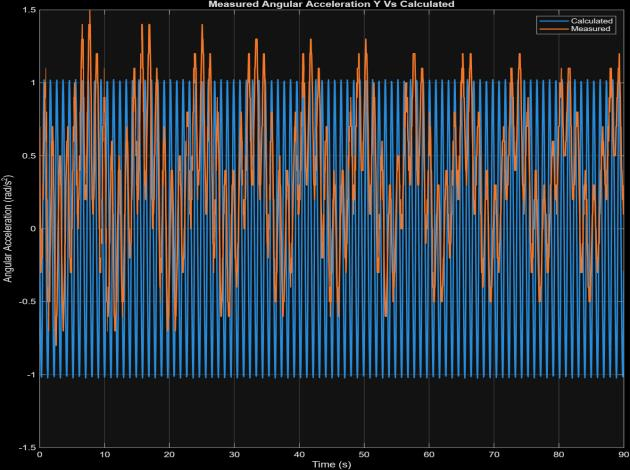
\includegraphics[width=\textwidth]{figures/acceleration_y_90s.png}
\caption{Full \SI{90}{s}.}
\end{subfigure}
\caption{Measured and calculated linear acceleration, sensor $y$ channel.}
\label{fig:ay}
\end{figure}

\begin{figure}[H]
\centering
\begin{subfigure}[t]{0.49\textwidth}
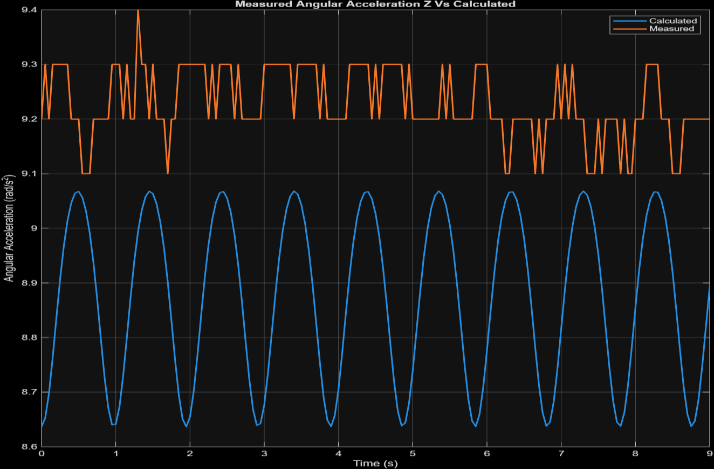
\includegraphics[width=\textwidth]{figures/acceleration_z_9s.png}
\caption{First \SI{9}{s}.}
\end{subfigure}\hfill
\begin{subfigure}[t]{0.49\textwidth}
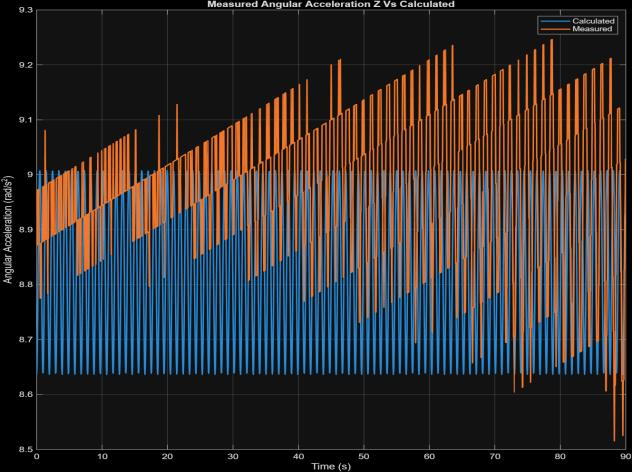
\includegraphics[width=\textwidth]{figures/acceleration_z_90s.png}
\caption{Full \SI{90}{s}.}
\end{subfigure}
\caption{Measured and calculated linear acceleration, sensor $z$ channel.}
\label{fig:az}
\end{figure}

\section{Discussion}
\subsection{What the model captures}
The simulation and physical apparatus precess in the same direction relative to the rotor spin, and both exhibit a nutation-like oscillation following release. In the short-duration comparisons, the simulated angular-velocity amplitudes and the measured signals have similar order and periodic structure. These observations indicate that the chosen coordinate sequence and dominant gravity-driven gyroscopic coupling are consistent with the physical system.

\subsection{Sources of discrepancy}
Several modeling choices explain why the curves do not remain coincident over \SI{90}{s}:
\begin{itemize}
    \item \textbf{Dissipation is omitted.} The physical rotor experiences bearing friction, aerodynamic drag, and other losses, whereas the simulation retains energy except for numerical integration effects.
    \item \textbf{Initial spin is estimated.} The rotor speed was approximated at \SI{500}{rpm}; even a modest error changes the precession rate and therefore accumulates phase error over time.
    \item \textbf{Geometry is simplified.} The rotor-pulley assembly is represented with an approximate combined center position, and the connecting rod is treated as massless.
    \item \textbf{Sensor behavior is idealized.} The original long-window acceleration data contain low-frequency structure not present in the model, especially in the $y$ channel. This could reflect sensor bias, acquisition behavior, alignment error, or unmodeled mechanical motion.
    \item \textbf{No parameter identification is performed.} The model uses measured/estimated geometry directly rather than fitting uncertain parameters to the experimental data.
\end{itemize}

A stronger next iteration would estimate rotor-speed decay from the data, include viscous or Coulomb friction, use an exact mass-weighted center of mass for the rotor-pulley assembly, and evaluate agreement with RMSE and phase-error metrics. These changes would convert the current qualitative validation into a more rigorous identification-and-validation workflow.

\section{Conclusion}
A nonlinear Newton--Euler model of a laboratory gyroscope was constructed using explicit rotation matrices, pivot-referenced inertia tensors, angular-momentum transport, and numerical integration in MATLAB. The simulation reproduces the primary direction and oscillatory structure of the measured precession and nutation. The remaining long-term differences are consistent with the model's deliberate idealizations, most importantly the absence of friction and the use of estimated initial conditions. The project demonstrates how classical rigid-body dynamics can be translated into a computational model and then evaluated against real sensor measurements rather than only visual motion.

For repository use, the project is best presented as a dynamics modeling and experimental-validation study: the analytical formulation, MATLAB implementation, and comparison plots together are more informative than the animation alone.

\section*{References}
\addcontentsline{toc}{section}{References}
\begin{thebibliography}{9}
\bibitem{openstax_precession}
OpenStax / Physics LibreTexts, ``Precession of a Gyroscope,'' \textit{University Physics I}, section 11.5, accessed in the original project via Physics LibreTexts.

\bibitem{kostov2011}
S. Kostov and D. Hammer, ``It Has to Go Down a Little, in Order to Go Around---Revisiting Feynman on the Gyroscope,'' \textit{The Physics Teacher}, vol. 49, no. 4, pp. 216--219, 2011. doi:10.1119/1.3566029.

\bibitem{openstax_centripetal}
OpenStax / Physics LibreTexts, ``Centripetal Acceleration,'' \textit{College Physics}, section 6.2, accessed in the original project via Physics LibreTexts.
\end{thebibliography}

\appendix
\section{Repository-Oriented File Layout}
A compact public repository can use the following structure:
\begin{lstlisting}
gyroscope-dynamics-simulation/
|-- README.md
|-- src/
|   `-- gyroscope_simulation.m
|-- report/
|   |-- gyroscope_dynamics_report.tex
|   |-- gyroscope_dynamics_report.pdf
|   `-- figures/
|-- data/
|   `-- README.md
`-- media/
    `-- README.md
\end{lstlisting}
The raw sensor CSV should be added only if the team has permission to publish it. Generated MATLAB videos and local data exports are better excluded from version control by default.

\end{document}
